%\documentclass{article}
%\documentclass[hyperref={colorlinks=true}]{beamer}
\documentclass[handout,hyperref={colorlinks=true}]{beamer}

\usecolortheme{crane}
\usetheme{Darmstadt}
\usefonttheme{structuresmallcapsserif}
%%%%%%%%%%%%%%%%%%%%%%%%%%%%%%Paquetes%%%%%%%%%%%%%%%%%%%%%%%%%%%%%%%%%%%%%%%%%%%%%%%5
%%%%%%%%%%%%%%%%%%%%%%%%%%%%%%%%%%%%%%%%%%%%%%%%%%%%%%%%%%%%%%%%%%%%%%%%%%%%%%%%%%%%%
%\usepackage{pgfpages}
%\pgfpagesuselayout{2 on 1}[a4paper,border shrink=5mm]
\usepackage{empheq}
\usepackage[spanish]{babel}
\usepackage[utf8x]{inputenc}
\usepackage{times}
\usepackage[T1]{fontenc}
\usepackage{amssymb,amsmath}
\usepackage{enumerate}
\usepackage{verbatim}
\usepackage{ esint }
%\usepackage{pst-all}
%\usepackage{pstricks-add}
\usepackage{array}
%\usepackage[T1]{fontenc}
\usepackage{animate}
%\usepackage{media9}
\usepackage{xparse}
\usepackage{listings}
\usepackage{ wasysym }
\usepackage{sagetex}
\usepackage{hyperref}
%%%%%%%%%%%%%%%%%%%%%%%%%Configuracion listing
\lstdefinelanguage{Sage}[]{Python}
{morekeywords={False,sage,True},sensitive=true}
\lstset{
frame=none,
showtabs=False,
showspaces=False,
showstringspaces=False,
commentstyle={\ttfamily\color{dgreencolor}},
keywordstyle={\ttfamily\color{dbluecolor}\bfseries},
stringstyle={\ttfamily\color{dgraycolor}\bfseries},
language=Sage,
basicstyle={\fontsize{8pt}{8pt}\ttfamily},
aboveskip=.3em,
belowskip=0.1em,
numbers=none,
numberstyle=\footnotesize
}

\AtBeginSection[]
{
  \begin{frame}
    \frametitle{Índice}
    \tableofcontents[currentsection]
  \end{frame}
}


%%%%%%%%%%%%%%%%%%%%%%%%Colores
\definecolor{myblue}{rgb}{.8, .8, 1}
\definecolor{dblackcolor}{rgb}{0.0,0.0,0.0}
\definecolor{dbluecolor}{rgb}{0.01,0.02,0.7}
\definecolor{dgreencolor}{rgb}{0.2,0.4,0.0}
\definecolor{dgraycolor}{rgb}{0.30,0.3,0.30}
\newcommand{\dblue}{\color{dbluecolor}\bf}
\newcommand{\dred}{\color{dredcolor}\bf}
\newcommand{\dblack}{\color{dblackcolor}\bf}
%%%%%%%%%%%%%%%%%%%%%%%%%%Nuevos comandos entornos%%%%%%%%%%%%%%%%%%%%%%%%%%%%%%%%
%%%%%%%%%%%%%%%%%%%%%%%%%%%%%%%%%%%%%%%%%%%%%%%%%%%%%%%%%%%%%%%%%%%%%%%%
\newenvironment{demo}{\noindent\emph{Dem.}}{$\square$ \newline\vspace{5pt}}
\newcommand{\com}{\mathbb{C}}
\newcommand{\dis}{\mathbb{D}}
\newcommand{\rr}{\mathbb{R}}
\newcommand{\oo}{\mathcal{O}}
\renewcommand{\emph}[1]{\textcolor[rgb]{1,0,0}{#1}}
\newcommand{\der}[2]{\frac{\partial #1}{\partial #2}}
\renewcommand{\v}[1]{\overrightarrow{#1}}
\renewcommand{\epsilon}{\varepsilon}
\newlength\mytemplen
\newsavebox\mytempbox
\makeatletter
\newcommand\mybluebox{%
\@ifnextchar[%]
{\@mybluebox}%
{\@mybluebox[0pt]}}
\def\@mybluebox[#1]{%
\@ifnextchar[%]
{\@@mybluebox[#1]}%
{\@@mybluebox[#1][0pt]}}
\def\@@mybluebox[#1][#2]#3{
\sbox\mytempbox{#3}%
\mytemplen\ht\mytempbox
\advance\mytemplen #1\relax
\ht\mytempbox\mytemplen
\mytemplen\dp\mytempbox
\advance\mytemplen #2\relax
\dp\mytempbox\mytemplen
\colorbox{myblue}{\hspace{1em}\usebox{\mytempbox}\hspace{1em}}}
\makeatother
\DeclareDocumentCommand\boxedeq{ m g }{%
{\begin{empheq}[box={\mybluebox[2pt][2pt]}]{equation}% #1%
\IfNoValueF {#2} {\label{#2}}%
#1
\end{empheq}
}%
}
\DeclareMathOperator{\atan2}{atan2}
\DeclareMathOperator{\sen}{sen}
\newtheorem{teorema}{Teorema}[section]
\newtheorem{lema}[teorema]{Lema}
\newtheorem{corolario}[teorema]{Corolario}
\newtheorem{proposicion}[teorema]{Proposici\'on}
\newtheorem{definicion}[teorema]{Definici\'on}
%%%%%%%%%%%%%%%%%%%%%%%%%%%%%%%%%%%%%%%%%%%%%%%%%%%%%%%%%%%%%%%%%%%%%%%%%%%%%%%%%%%%%%%%%%%%%%%%%%%%%%%%%%%
%%%%%%%%%%Para escibir en clase articulo o similar
% \usepackage{color}
% \newcommand{\nl}{ }
% \renewenvironment{frame}[1]{}{}
% \newcommand{\qed}{$\square$}
% %\newcommand{\defverbatim}{\def{#1}}
% \newenvironment{block}[1]{\textbf{#1}}{}
% \title{Ecuaciones lineales de segundo orden}
% \author{Fernando Mazzone}
%
%%%%%%%%%%%%%%%%%%%%%%%Para clase beamer
\newcommand{\nl}{\onslide<+-> }

\title[Ecuaciones de primer orden] % (optional, nur bei langen Titeln nötig)
{%
 Ecuaciones de primer orden
}

\date{}

%\author[] % (optional, nur bei vielen Autoren)
%{Fernando Mazzone}

%\institute[Depto de Matemática] % (optional, aber oft nötig)
%{
% Depto de Matemática\\
%Facultad de Ciencias Exactas Físico-Químicas y Naturales\\
%Universidad Nacional de Río Cuarto}


\subject{Ecuaciones Diferenciales}

%%%%%%%%%%%%%%%%%%%%%%%%%%%%%%%%%%%%%%%%%%%%%%%%%%%%%%%%%%%%%%%%%%%%%%%%%%%%%%%%%%%%%%





\begin{document}

\begin{frame}
  \maketitle
  \begin{center}
   
\includegraphics[scale=0.2]{imagenes/unrc.jpg}
   \end{center}
\end{frame}





\begin{frame}
  \frametitle{Índice}
\tableofcontents
\end{frame}










\section[Homogéneas]{Ecuaciones homogéneas}

\begin{frame}{Ecuaciones homogéneas}

\nl\begin{block}{Funciones homogéneas}
 Una función $F:\rr\times\rr\to\rr$ se dice homogénea de grado $\alpha$ si 
 \[f(rx,ry)=r^{\alpha}f(x,y).\]
\end{block}
\textbf{Ejemplos}
\begin{itemize}
                 \nl\item $f(x,y)=\tfrac{y}{x}$ es homogénea de grado $0$.
                \nl \item Más generalmente, cualquier función $f(x,y)$ que dependa sólo de $x/y$, esto es que se escriba de la forma $f(x,y)=g(y/x)$
                 es homogénea de grado  $0$. Así $f(x,y)=\tfrac{x-y}{x+y}$ es homogénea de grado $0$ pues $\tfrac{x-y}{x+y}= \tfrac{1-x/y}{1+x/y}$
                \nl \item $f(x,y)=\sum_{k=0}^na_kx^ky^{n-k}$ es homogénea de grado $n$.
\end{itemize}

\end{frame}

\begin{frame}{Ecuaciones homogéneas}

\nl\begin{block}{Resolviendo ecuaciones homogéneas}
 Una ecuación 
 \begin{equation}\label{ecua_prin}y'=f(x,y)\end{equation}
 tal que $f$ es homogénea de grado $0$ se llamará ecuación homogénea.
\end{block}

\nl\begin{block}{Resolviendo ecuaciones homogéneas}
 Si una ecuación del tipo \eqref{ecua_prin} es homogénea entonces se transforma en una ecuación separable mediante el cambio de variable dependiente $\boxed{z=y/x}$.
\end{block}


\end{frame}


\begin{frame}{Resolviendo ecuaciones homogéneas}

En efecto, para $x\neq 0$

\[f(x,y)=x^0f\left(1,\frac{y}{x}\right)=f(1,z)\]
y
\[y'=z'x+z\]
Como $y'=f(x,y)$ tenemos
\begin{equation}\label{cambio_hom}z'x+z=f(1,z)\Longrightarrow \frac{dz}{f(1,z)-z}=\frac{dx}{x}.\end{equation}
\end{frame}

\begin{frame}{Resolvieno ecuaciones homogéneas}
\textbf{Ejemplo} Resolver $y'=\frac{x+y}{x-y}$. 

La ecuación \eqref{cambio_hom} queda
\[ \begin{array}{c} \frac{dx}{x}=\frac{dz}{\frac{1+z}{1-z}-z}=\frac{(1-z)dz}{1+z^2}\\
 \Downarrow\\
\ln|x|+C=\arctan(z)-\frac{1}{2}\ln|1+z^2|
    \end{array}.
\]



\end{frame}

\section[Exactas]{Ecuaciones exactas}

\begin{frame}{Ecuaciones exactas}

\begin{block}{Definición}
\nl Dada una función $f$ de $n$ variables independientes $x_1,\ldots,x_n$ definimos su \href{http://es.wikipedia.org/wiki/Diferencial_de_una_función}{diferencial}
 por 
 \[df=\frac{\partial f}{\partial x_1}dx_1+\cdots +\frac{\partial f}{\partial x_n}dx_n.\]
\end{block}

\nl Es costumbre escribir las ecuaciones diferenciales   de la siguiente forma, supongamos  $f(x,y)=-M(x,y)/N(x,y)$
entonces
\[y'=-\frac{M(x,y)}{N(x,y)}\leftrightarrows M(x,y)dx+N(x,y)dy=0.\] 


\end{frame}

\begin{frame}{Ecuaciones exactas}
\nl Dada $f:\rr\times\rr\to\rr$ la familia paramétrica de curvas
\[f(x,y)=c\]
satisface a ecuación diferencial

\[
 \frac{\partial f}{\partial x}+\frac{\partial f}{\partial y}y'=0\Longleftrightarrow \frac{\partial f}{\partial x}dx+\frac{\partial f}{\partial y}dy=0
 \Longleftrightarrow df=0.
\]
\nl El recíproco es tambien cierto, esto es una ecuación que se puede expresar como $df=0$  tiene soluciones dadas por la familia paramétrica de arriba. 

\nl Para que una ecuación cualquiera
\[M(x,y)dx+N(x,y)dy=0\]
Se pueda expresar como $df=0$ se debe cumplir que debe existir $f(x,y)$ tal que $M=\partial f/\partial x$ y $N=\partial f/\partial y$.
\end{frame}

\begin{frame}{Ecuaciones exactas}\label{camposconservativos}
\nl Vale decir el campo vectorial $(x,y)\mapsto (M(x,y),N(x,y))$ es un \href{http://es.wikipedia.org/wiki/Fuerza_conservativa}{campo 
gradiente o conservativo} con potencial $f$. No todo campo es un campo gradiente, recordemos

\nl \begin{block}{Caracterización de campos conservativos}Sea $\mathcal{O}$ abierto de $\rr^n$ y simplemente conexo. Son equivalentes
 \begin{enumerate}
  \item El campo $F:\mathcal{O}\to\rr^n$ es un gradiente.
  \item Si $C$ es un camino cerrado entonces
  \[\varointctrclockwise_C F\cdot d x=0.\]
  \item\label{item1} \[\frac{\partial F^i}{\partial x_j}=\frac{\partial F^j}{\partial x_i},\quad\text{ para }i,j=1,\ldots,n\]. 
 \end{enumerate}

\end{block}

\end{frame}

\begin{frame}{Ecuaciones exactas}
El item \ref{item1}  es particularmente simple de chequear. Una vez establecido con un campo es conservativo tendremos el problema de hallar el potencial $f$. 
Ilustremos esto con el campo $(x,y)\mapsto (M(x,y),N(x,y))$. Supongamos que $\mathcal{O}$ es abierto de $\rr^2$ y
\[\frac{\partial M}{\partial y}=\frac{\partial N}{\partial x},\quad\text{ para } (x,y)\in \mathcal{O}.\] 
En primer lugar debemos tener un campo escalar $f$ tal que
\[M=\frac{\partial f}{\partial x}\Rightarrow f=\int Mdx +C(y).\]
Ahora como $f_y=N$
\[N=\frac{\partial f}{\partial y}=\frac{\partial}{\partial y}\int Mdx +C'(y).\]

\end{frame}

\begin{frame}{Ecuaciones exactas}
\[C'(y)=N-\frac{\partial}{\partial y}\int Mdx .\]
\nl Para que esta ecuación tenga solución $N-\frac{\partial}{\partial y}\int Mdx$ debe ser sólo función de $y$. Pero la condición necesaria y suficiente para ello es 
\[\begin{split}0&=\frac{\partial}{\partial x}\left(N-\frac{\partial}{\partial y}\int Mdx\right)\\
&= \der{N}{x}-\frac{\partial^2}{\partial x\partial y}\int Mdx\\
&=\der{N}{x}-\frac{\partial^2}{\partial y\partial x}\int Mdx\\
&=\der{N}{x}-\der{M}{y}.
   \end{split}
\]
\end{frame}

\begin{frame}{Ecuaciones exactas}
\nl Pero estamos bajo ese supuesto, entonces
\boxedeq{C(y)=\int\left( N-\frac{\partial}{\partial y}\int Mdx \right)dy.}

\nl\textbf{Ejemplo} Resolver $e^ydx+(xe^y+2y)dy=0$. 

\nl\textbf{Solución} Aquí
\[M=e^y\quad\text{ y }N=xe^y+2y.\]
Así
\[\der{M}{y}=e^y=\der{N}{x}.\]
La ecuación es exacta. El potencial $f$ debe cumplir
\[f=\int e^ydx=xe^y+C(y)\]


\end{frame}


\begin{frame}{Ecuaciones exactas}
y
\[C(y)=\int\left( xe^y+2y -\frac{\partial}{\partial y} xe^y\right)dy= y^2\]
Tener en cuenta que la función potencial $f$ no es única, queda deerminada hasta una constante aditiva de integración que podemos elegir a gusto ya que 
debemos encontrar sólo un potencial. Entonces podemos tomar
\[f= xe^y+y^2.\]
La solución general de la ecuación estará dada por
\[xe^y+y^2=c,\quad c\in\rr.\]
Como no sabemos despejar $\boxed{y}$ de aquí dejamos indicada de esta manera la solución.

\end{frame}

\section{Factores integrantes}
\begin{frame}{Factores integrantes}
\nl Las ecuaciones exactas son raras, no obstante tenemos un recurso para llevar algunas ecuaciones no exactas a una equivalente y exacta.

\nl Supongamos que la ecuación
\[Mdx+Ndy=0\]
no es  exacta. La idea es econtrar una función $\mu(x,y)$ llamada 
\href{http://es.wikipedia.org/wiki/Ecuación_diferencial_exacta\#Factor_integrante.}{factor integrante} que haga que la ecuación
\[\mu\left(Mdx+Ndy\right)=0\]
si lo sea. Para ello se debe cumplir que
\begin{equation}\label{carac_factor}
  \der{\mu M}{y}=\der{\mu N}{x}\Longleftrightarrow \boxed{ \mu\der{M}{y}+\der{\mu}{y}M=\der{N}{x}\mu+N\der{\mu}{x}}.
\end{equation}
 
\end{frame}
 
 
\begin{frame}{Factores integrantes}
 \begin{block}{Observación}
  Toda ecuación
  \begin{equation}\label{ec_no_exa}Mdx+Ndy=0
   \end{equation}
  que tiene una solución general que se escribe
  \begin{equation}\label{sol_ec_no_exa}
   f(x,y)=c,  
  \end{equation}
  tiene, en teoría, un factor integrante. 
 \end{block}

 
 
 
\end{frame}

\begin{frame}{Factores integrantes}
Si derivamos \eqref{sol_ec_no_exa}
\[\der{f}{x}dx+\der{f}{y}dy=0.\]
De esta ecuación y \eqref{ec_no_exa} vemos que
\[-\frac{M}{N}=y'=-\frac{\partial f /\partial x}{\partial f/\partial y}\Longrightarrow \frac{ \partial f /\partial x}{M}=\frac{ \partial f/\partial y}{N}=:\mu(x,y)\]
Aquí hemos asumido $N\neq 0 \neq\der{f}{y}$. De la igualdad de arrriba se deduce que existe $\mu(x,y)$ con
\[\der{f}{x}=\mu M\quad\text{ y }\quad \der{f}{y}=\mu N.\]
Es decir $\mu$ es factor integrante.
\end{frame}

\begin{frame}{Factores integrantes}
La observación nos dice que parece razonable que siempre exista un factor integrante, pero no ayuda a hallarlo puesto que deberíamos conocer la solución general de la ecuación
para hacerlo. O deberíamos resolver la ecuación \eqref{carac_factor} que es una ecuación en derivadas parciales para $\mu$.

Hay que señalar que sólo necesitamos una solución de \eqref{carac_factor} y no su solución general. En la práctica se suele proceder a hacer alguna suposición
sobre $\mu$ que simplifique la expresión (\href{http://es.wikipedia.org/wiki/Ansatz}{ansatz}). Es común suponer que $\mu$ es sólo función de una de las variables. Si por ejemplo asumimos que $\mu=\mu(x)$ las ecuaciones 
\eqref{carac_factor} se escriben

\[\mu\der{M}{y}=\mu\der{N}{x}+N\mu'(x) \Longrightarrow\boxed{\frac{\mu'}{\mu}=\frac{\partial M/\partial y-\partial N/\partial x}{N}}\]
\end{frame}


\begin{frame}{Factores integrantes}
Para que esto funcione la función 

\[\frac{\partial M/\partial y-\partial N/\partial x}{N}\]

\emph{debe depender sólo de $x$}. Si eso ocurre y llamamos $h(x)$ a esa función vamos a tener que
\[\mu(x)=e^{\int h(x)dx}\]
es un factor integrante. Recordar que sólo necesitamos hallar uno, por ese motivo no consideramos constantes de integración. 
\end{frame}

\begin{frame}{Factores integrantes}
De manera similar, si la función
\[\frac{\partial M/\partial y-\partial N/\partial x}{-M}\]
depende sólo de $y$ y llamamos $h(y)$ a esa función tenemos que
\[\mu(y)=e^{\int h(y)dy}\]
es un factor integrante, que en este caso sólo depende de $y$.
\end{frame}

\begin{frame}{Factores integrantes}
\textbf{Ejemplo 1} $ydx+(x^2y-x)dy=0$.
Primero chequeemos la posible exactitud.
\[\der{M}{y}=1\text{ y } \der{N}{x}=2xy-1\Longrightarrow\text{no exacta}.\]
Ahora 
\[\frac{\partial M/\partial y-\partial N/\partial x}{N}=\frac{2-2xy}{x(xy-1)}=-\frac{2}{x}=:h(x).\]
El factor integrante es
\[\mu(x)=e^{\int h(x)dx}=e^{-2\ln |x|}=\frac{1}{x^2}.\]

\end{frame}


\begin{frame}{Exactitud, Otras Técnicas}

Veamos otra forma de trabajar para transformar ecuaciones no exactas en exactas. Aunque esta forma no es metódica, sino  que depende de la habilidad 
de quien la lleva adelante. Consiste en explotar la similitud de la ecuación diferencial con alguna expresión exacta conocida. Ilustremos esto con el ejemplo anterior 
$ydx+(x^2y-x)dy=0$. La ecuación equivale a
\[x^2ydy-(xdy-ydx)=0.\]
Ahora podemos notar que 
\[d\left(\frac{y}{x}\right)=\frac{xdy-ydx}{x^2}.\]
Lo que sugiere dividir por $x^2$ la ecuación.

\end{frame}

\begin{frame}{Exactitud, Otras Técnicas}

\[0=ydy-\frac{xdy-ydx}{x^2}=d\left(\frac{y^2}{2}\right)-d\left(\frac{y}{x}\right)=d\left(\frac{y^2}{2}-\frac{y}{x}\right).\]
La solución general es pues
\[\frac{y^2}{2}-\frac{y}{x}=c.\]

\end{frame}

\begin{frame}{Exactitud, Otras Técnicas}

Otras fórmulas para tener en cuenta que son exactas
%\begin{equation}
 \begin{align}
  d\left(\frac{x}{y}\right)&=\frac{ydx-xdy}{y^2}\quad\text{nada nuevo} \\
  d(xy)&=ydx+xdy\\
  d(x^2+y^2)&=2(xdx+ydy)\label{eq:exacta_mod2}\\
  d\left( \arctan\left(\frac{y}{x} \right) \right)&=\frac{ydx-xdy}{x^2+y^2}\quad\text{falla caracterización pag \ref{camposconservativos}!!!!}\nonumber\\
  d\left( \ln\left(\frac{y}{x} \right) \right)&=\frac{ydx-xdy}{xy}
  \end{align}
%\end{equation}


\end{frame}

\begin{frame}{Ejemplo, óptica}
\nl\begin{tabular}{m{5cm} m{4.5cm} }
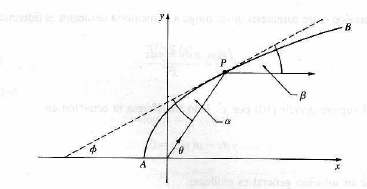
\includegraphics[scale=.4]{imagenes/espejo.png} & \textbf{Problema} Hallar la forma del espejo curvo tal que el reflejo de todo haz de luz que viaja paralelo al eje $x$ con dirección
negativa repecto a este eje pasa por el $(0,0)$. \\
\end{tabular}
\nl \textbf{Ejercicio} Dejamos como ejercicio demostrar que un haz de luz que se refleja sobre un espejo lo hace de tal manera que los ángulos que se forman con los rayos 
de incidencia y refracción y la tangente al espejo en el punto de incidencia son iguales ( $\beta=\alpha$ en el dibujo). Para resolver esto hay que usar el principio
de mínimo tiempo de Fermat


\end{frame}


\begin{frame}{Ejemplo, óptica}
 \textbf{Solución.} Sea $(x,y)$ el punto de incidencia. Apelando a la geometría elemental, $\phi=\beta$ y $\theta=\alpha+\phi=2\beta$. Como $\tan\theta=\frac{y}{x}$
  y como
  \[\tan\theta =\tan 2\beta=\frac{2\tan\beta}{1-\tan^2\beta},\]
deducimos que
\[\frac{y}{x}=\frac{2 dy/dx}{1-(dy/dx)^2}.\]
Despejando
\[\frac{dy}{dx} =\frac{-x\pm\sqrt{x^2+y^2}}{y}.\]

\end{frame}


\begin{frame}{Ejemplo, óptica}
Podemos escribir la ecuación de este otro modo
\[xdx+ydy=\pm\sqrt{x^2+y^2}dx.\]
Tomando en cuenta \eqref{eq:exacta_mod2}
\[\pm\frac{d(x^2+y^2)}{2\sqrt{x^2+y^2}}=dx.\]
Si $r=x^2+y^2$
\[dx=\pm\frac{dr}{2\sqrt{r}}=\pm d\sqrt{r}=\pm d\sqrt{x^2+y^2}\]
Las solución general es
\[\pm\sqrt{x^2+y^2}=x+c.\]
 


\end{frame}


\begin{frame}{Ejemplo, óptica}
 \begin{tabular}{m{4cm} m{5cm}}
 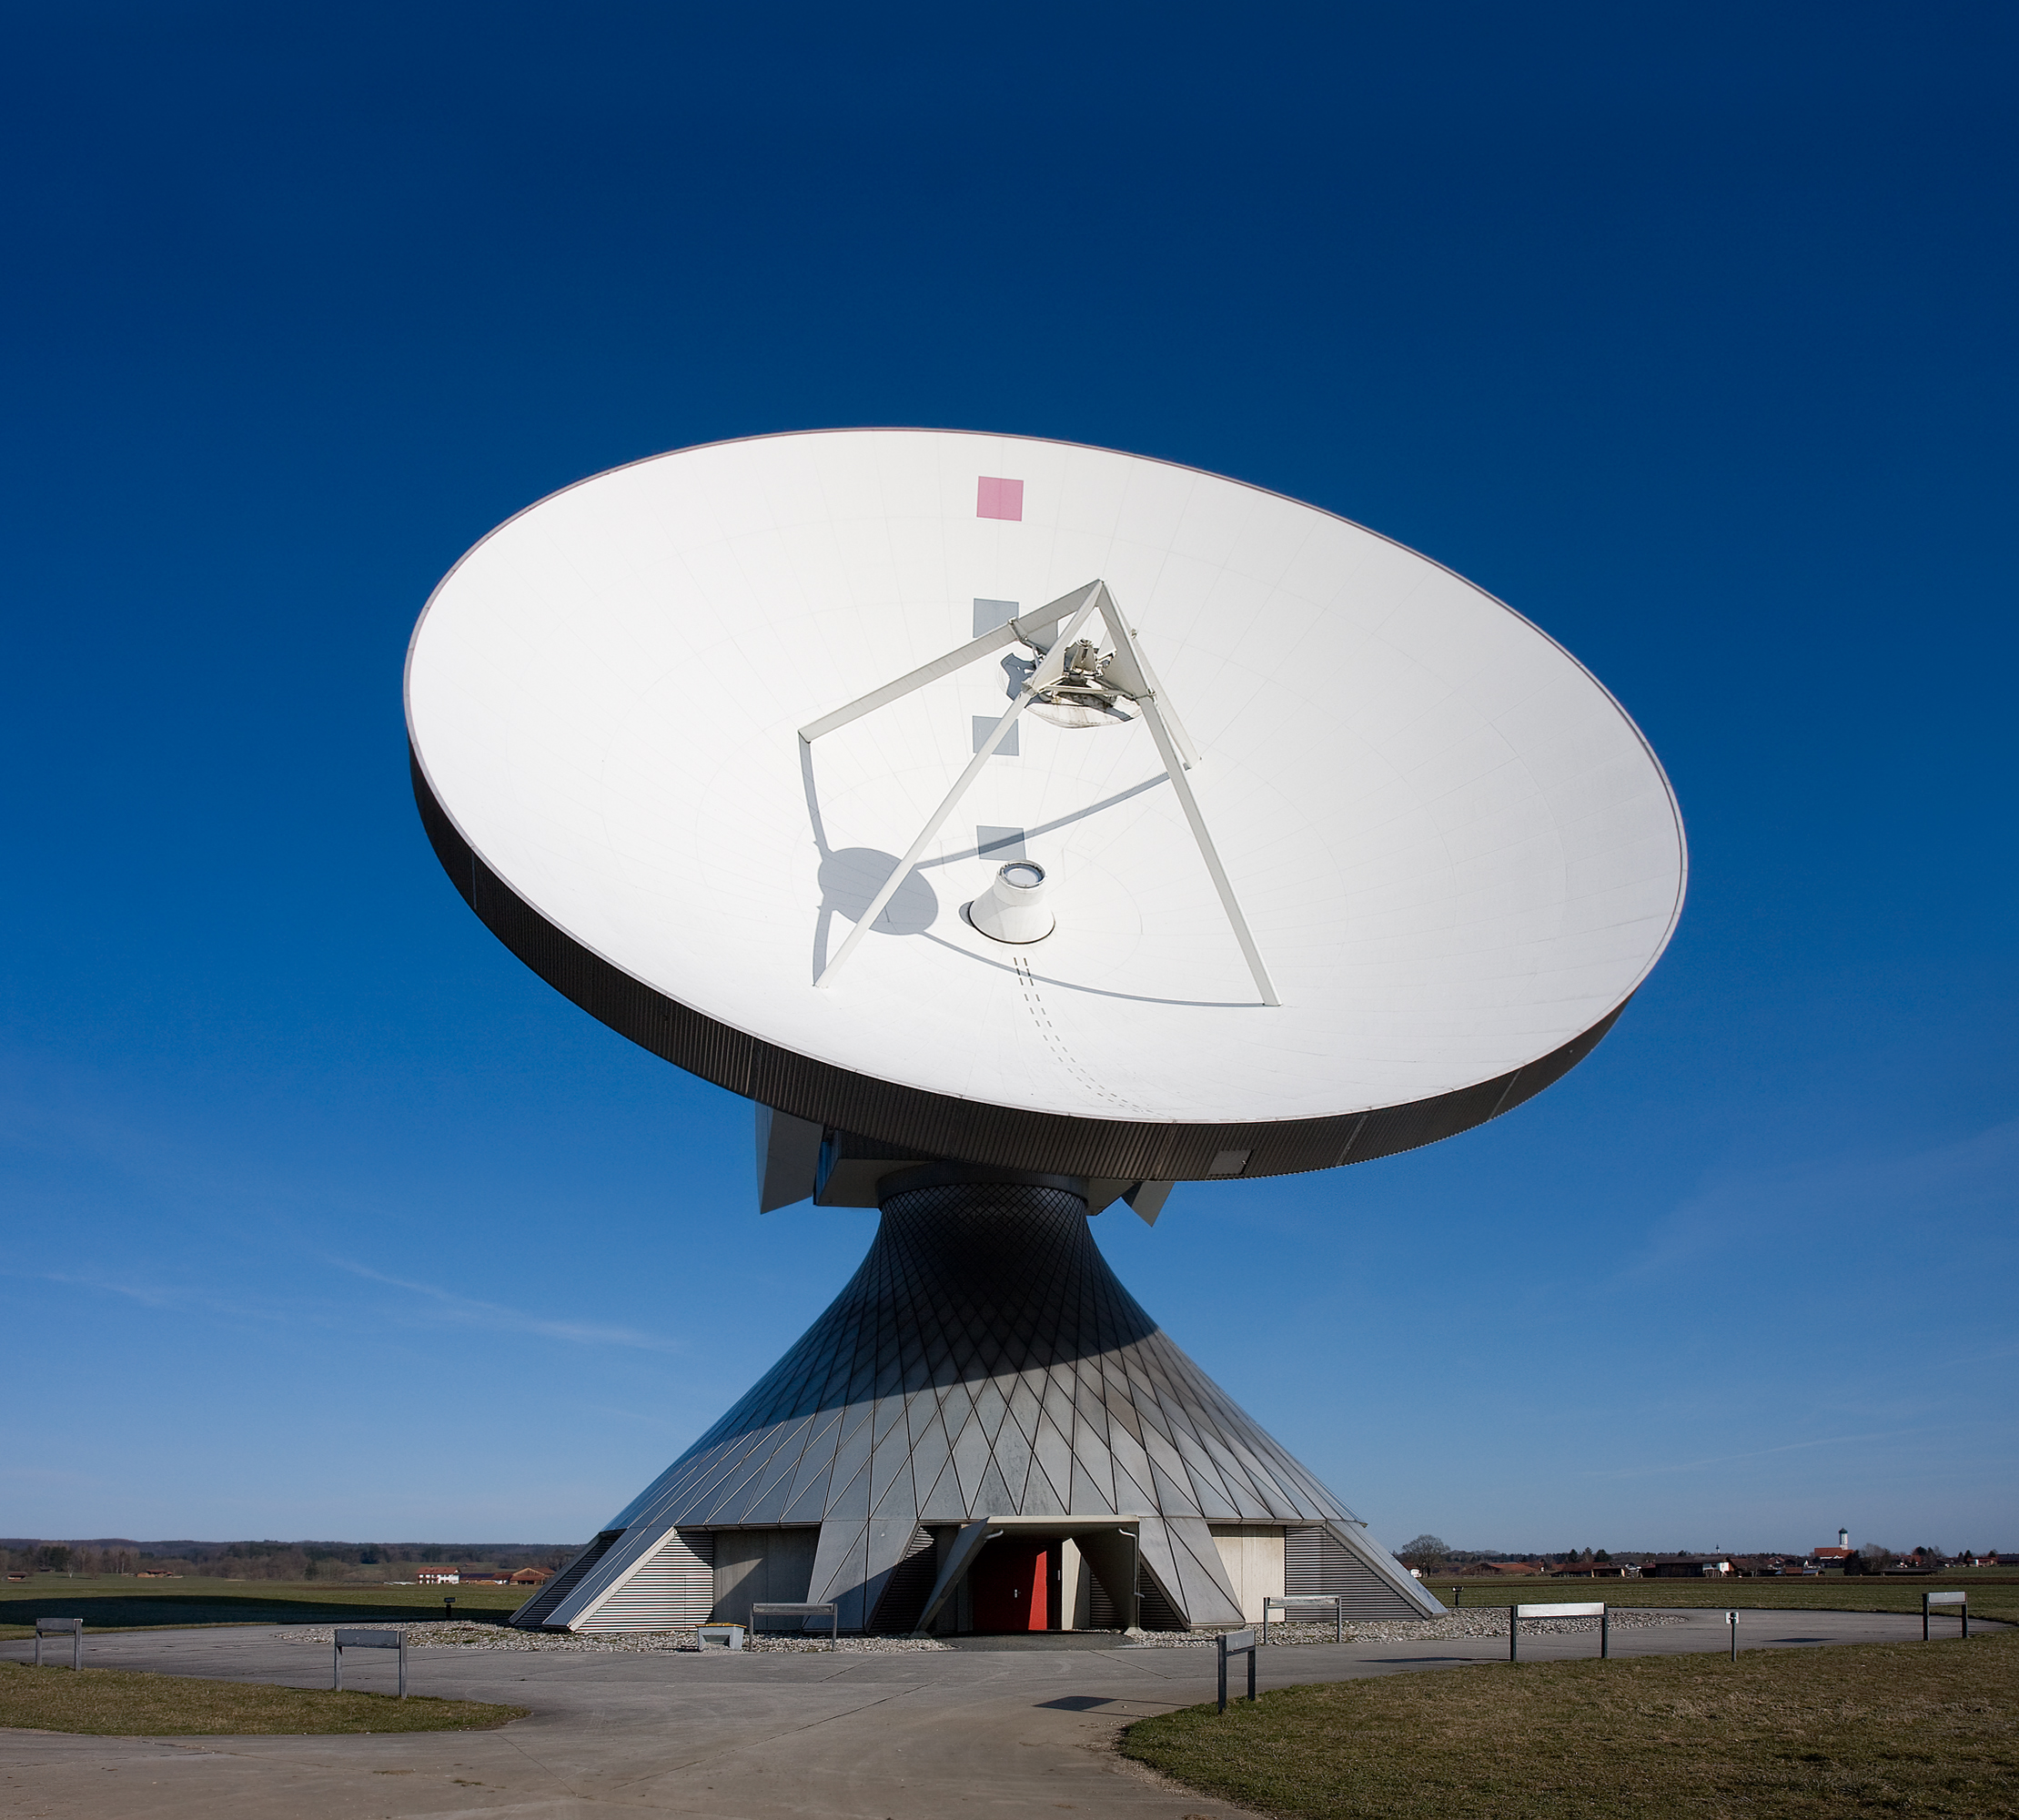
\includegraphics[scale=.15]{imagenes/antena.jpg} & Elevando al cuadrado ambos miembros
\[y^2=2xc+c^2=2c\left(x+\frac{c}{2}\right)\]
Que es la familia de todas las parábolas con eje de simetría $x$, positivamente orientadas y con foco en $(0,0)$. \\
 \end{tabular}
 \end{frame}
\section[Lineales]{Ecuaciones Lineales}

\begin{frame}{Ecuaciones Lineales}
Se llama \href{http://es.wikipedia.org/wiki/Ecuación_diferencial_lineal}{ecuación diferencial lineal} a una ecuación que es lineal
respecto a   la/s variables
dependientes. La ecuación puede ser no lineal repecto a la variable independiente. 
La siguiente es la ecuación diferencial lineal general de primer orden
\begin{equation}\label{eq:lineal}y'+p(x)y=q(x).
\end{equation}
y la  de segundo orden
\[y''+p(x)y'+q(x)y=r(x).\]
Es costumbre introducir los operadores  $L_1[y]=y'+py$  y $ L_2[y]=y''+py'+qy$. 
Haciendo más precisa la definición, los operadores $L_1$ y $L_2$ son lineales, es decir, por ejemplo, $L_1[y_1+y_2]=L_1[y_1]+L_1[y_2]$. 
\end{frame}

\begin{frame}{Ecuaciones Lineales}
 Vamos a resolver la ecuación lineal de primer orden \eqref{eq:lineal}. Esto es sencillo pues la ecuación equivalente
 \begin{equation}\label{eq:lineal2}dy+(p(x)y-q(x))dx=0
  \end{equation}
tiene un factor integrante. En efecto como $M=p(x)y-q(x)$ y $N=1$. 
 \[\frac{\mu'}{\mu}=\frac{\partial M/\partial y-\partial N/\partial x}{N}=p(x).\]
 Entonces $\mu(x)=e^{\int pdx}$ es factor integrante. Luego si multiplicamos por $\mu$ en \eqref{eq:lineal2},  la expresión  es exacta. 
 \[e^{\int pdx}dy+p(x)e^{\int pdx}ydx=q(x)e^{\int pdx}dx.\]
\end{frame}

\begin{frame}{Ecuaciones Lineales}
Podemos identificar rápidamente, sin necesidad de hacer cálculos, el correspondiente potencial.
 \[d\left(e^{\int pdx}y\right)=d\left(\int q(x)e^{\int p} dx \right).\]
Integrando
\[e^{\int pdx}y=\int e^{\int pdx}q(x)dx+C.
 \]
 O
 \boxedeq{y=e^{-\int pdx}\left\{\int e^{\int pdx}q(x)dx+C\right\} }{SolGenLin}
 
 
 
 
\end{frame}


\begin{frame}{Ecuaciones Lineales}
\textbf{Ejemplo} Resolver $y'+y/x=3x$. 

\textbf{Solución.} En la práctica, para evitar recordar fórmulas, se suele repetir el procedimiento que llevo a la fórmula \eqref{SolGenLin}, ahora, dado la cercanía
de su derivación, vamos a usarla  de manera directa. La solución general es

\[\begin{split} y(x)&=e^{-\int\frac{1}{x}dx}\left\{\int e^{\int\frac{1}{x}dx}3xdx+C\right\}\\
   &=\frac{1}{|x|}\left\{\int |x| 3xdx+C\right\}\\
   &=x^2+\frac{C}{|x|}\\
   &=x^2+\frac{C}{x}\\
  \end{split}
\]
 
\end{frame}


\section{Reducción de orden}
\begin{frame}{Caso $F(x,y',y'')=0$}
Algunas ecuaciones de segundo orden
\boxedeq{F(x,y,y',y'')=0}{Gen2Or}
se pueden reducir a una de primer orden. Por ejemplo si $F$ no depende de $y$. Es decir la ecuación es
\boxedeq{F(x,y',y'')=0}
Aquí introducimos la nueva variable dependiente $\boxed{p=y'}$, que resuelve
\[F(x,p,p')=0.\]
Que es una ecuación de primer orden. Supuesto que la podemos resolver y encontrar una solución general para  $p$, tendremos
 

\end{frame}

\begin{frame}{Caso $F(x,y',y'')=0$}
 
\boxedeq{y=\int pdx+C}
Es la solución general de la ecuación de segundo orden.

\end{frame}

\begin{frame}{Caso $F(y,y',y'')=0$}\label{reduc_orden}
Si la ecuación general de segundo orden \eqref{Gen2Or} no depende de $x$, entonces nuevamente $\boxed{p=y'}$ como nueva variable depeniente
pero también usamos $\boxed{y}$ como nueva variable independiente. Como
\[y''=p'=\frac{dp}{dx}=\frac{dp}{dy}\frac{dy}{dx}=\frac{dp}{dy}p\]
La ecuación se reduce ala ecuación de primer orden
\boxedeq{F\left(y,p,\frac{dp}{dy}\right)=0}{RedOrdSinInd}

\end{frame}

\section{\texttt{SymPy}}



\begin{frame}[fragile]{\texttt{SymPy}: Clasificación de EDO}
\textbf{Sintaxis:} \verb+classify_ode(Eq)+

Donde
\verb+Eq+: es la ecuación.

El output son los métodos que se le pueden aplicar
\begin{sageblock}
from sympy import *
x=symbols('x')
y=Function('y')(x)
classify_ode(y.diff()+y)
\end{sageblock}

\verb+('separable', '1st_exact','1st_linear',+

\verb+'almost_linear','1st_power_series','lie_group',+


\verb+'nth_linear_constant_coeff_homogeneous', +

\verb+'separable_Integral', '1st_exact_Integral',  +

\verb+'1st_linear_Integral','almost_linear_Integral')+

\end{frame}

\begin{frame}[fragile]{\texttt{SymPy}: Clasificación de EDO}
\textbf{Sintaxis:} \verb+classify_ode(Eq)+

Donde
\verb+Eq+: es la ecuación.

El output son los métodos que se le pueden aplicar
\begin{sageblock}
Ecuacion=Eq((x**2*y-x)*sin((y.diff(x,1)))**3\
+y**5+x**3*sin(y),0)
classify_ode(Ecuacion)
\end{sageblock}

El único método que puede aplicar \texttt{SymPy} a la ecuación 

\[\sage{Ecuacion}\]

Es \verb+('lie_group',)+
\begin{sageblock}
dsolve(Ecuacion,y)
\end{sageblock}
Piensa, piensa   pero no llega a nada.
\end{frame}

\begin{frame}[fragile]{\texttt{SymPy: dsolve} }

\begin{lstlisting}
>>>Ecuacion=Eq(y.diff()+(-x+sqrt(x**2+y**2))/y,0)
>>>classify_ode(Ecuacion)
('1st_homogeneous_coeff_best', 
'1st_homogeneous_coeff_subs_indep_div_dep', 
'1st_homogeneous_coeff_subs_dep_div_indep', 
'1st_power_series', 'lie_group', 
'1st_homogeneous_coeff_subs_indep_div_dep_Integral', 
'1st_homogeneous_coeff_subs_dep_div_indep_Integral')
\end{lstlisting}

\begin{lstlisting}
>>>dsolve(Ecuacion,y,hint='lie_group')
\end{lstlisting}
Piensa rato largo y:
\begin{lstlisting}
The given ODE (-x + sqrt(x**2 + y(x)**2))/y(x) + Derivative(y(x), x) 
cannot be solved by the lie group method
\end{lstlisting}


\begin{lstlisting}
>>>sol=dsolve(Ecuacion,y,hint='1st_homogeneous_coeff_best')
\end{lstlisting}

\[y{\left (x \right )} = C_{1} e^{\int^{\frac{x}{y{\left (x \right )}}} -\frac{u_{2}}{u_{2}^{2} - u_{2} \sqrt{u_{2}^{2} + 1} - 1}\, du_{2} + \int^{\frac{x}{y{\left (x \right )}}} \frac{\sqrt{u_{2}^{2} + 1}}{u_{2}^{2} - u_{2} \sqrt{u_{2}^{2} + 1} - 1}\, du_{2}}\]

\end{frame}

\section[Ejemplos]{Ejemplos}


\begin{frame}{Velocidad de escape}\label{pag:vel_esc}

\begin{tabular}{m{4cm} m{5cm}}
 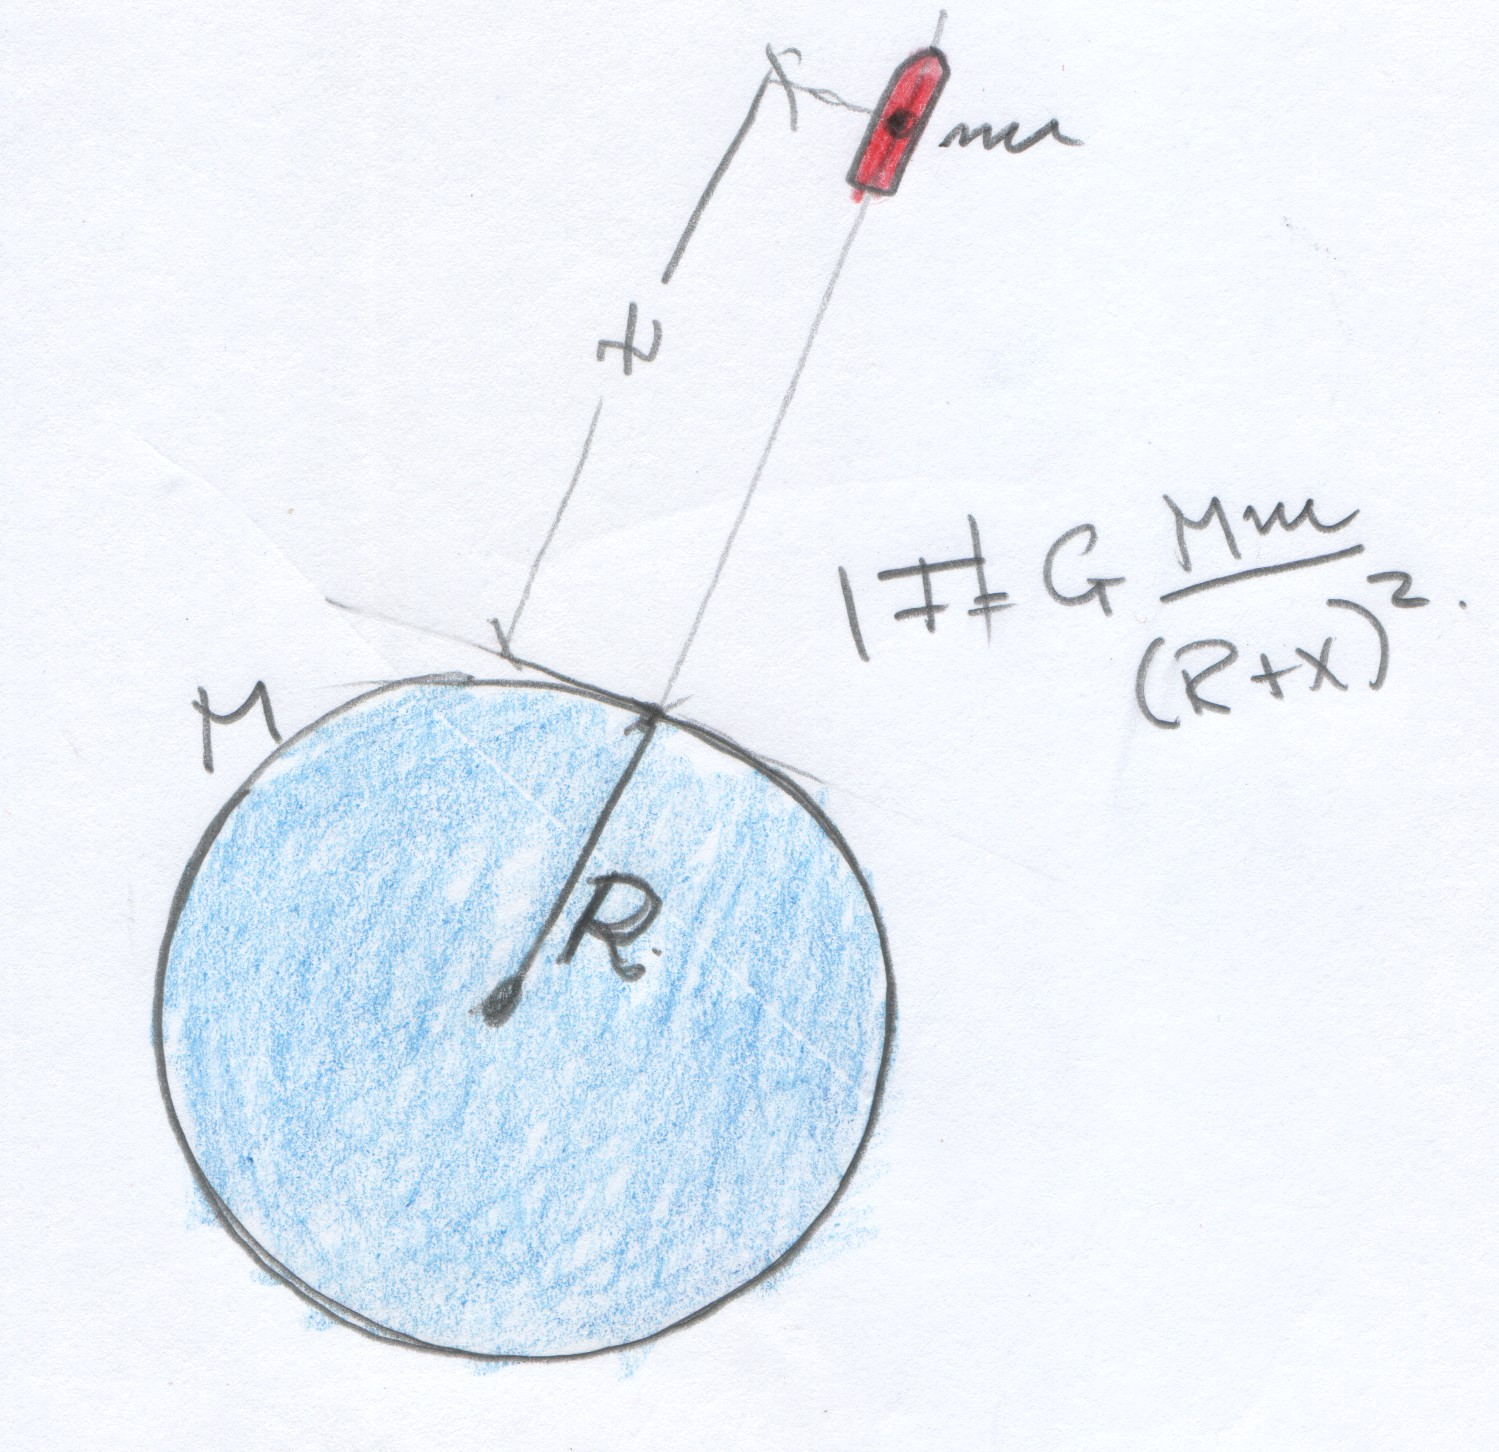
\includegraphics[scale=.075]{imagenes/tiro_vertical.jpg}&\textbf{Problema.} Que velocidad hay que imprimirle a un proyectil que es lanzado verticalmente desde la superficie de la Tierra si nuestra pretensión
es que el proyectil se escape al infinito. La velocidad más chica con esta cualidad se llama 
\href{http://es.wikipedia.org/wiki/Velocidad_de_escape}{velocidad de escape}.\\
\end{tabular}
 


\end{frame}

\begin{frame}{Velocidad de escape}
\textbf{Solución.} Para resolver este problema hay que tomar en consideración la 
\href{http://es.wikipedia.org/wiki/Ley_de_gravitación_universal}{Ley de gravitación universal} de Newton. En la parte que nos interesa, esta Ley afirma
que el módulo de la fuerza de gravedad que se ejercen entre si dos cuerpos de masa $m_1$ y $m_2$ separados una distancia $r$ es proporcional al producto de las masas  
e inversamente proporcional al cuadrado de las distancia que los separa. Vale decir
\[|F|=G\frac{m_1m_2}{r^2},\]
donde $G$ es la constante de proporcionalidad.
Cuando los cuerpos no son puntos masa, sino cuerpos extendidos en el espacio, la distancia de separación hay que medirla entre los centros de masa de los cuerpos. 
\end{frame}


\begin{frame}{Velocidad de escape}
Hay que aclarar que usando el \href{https://docs.google.com/file/d/0B80iJ0HgObRRWll6MlJFSjFNMGc/edit}{Principio conservación energía mecánica} podemos resolver
el problema de una manera más simple. Incluso podemos ver que la suposición de que el tiro es vertical no es necesaria, es decir la velocidad e escape es la misma aunque
el tiro sea oblicuo. Discutiremos esa solución durante la clase. Lamentablemente (o no)  esta solución no usa ecuaciones diferenciales.
Vamos a dar una solución, quizás un poco más complicada, pero que invoca las técnicas 
discutidas.

 

\end{frame}

\begin{frame}{Velocidad de escape}
 

Supondremos a la Tierra una esfera de radio $R$, masa $M$ y su centro de masa en el centro de la esfera.   Al proyectil lo supondremos un punto masa 
con masa $m$ y su posición en el momento $t$, denotada $x=x(t)$, la mediremos sobre un eje vertical con origen en la superficie de la Tierra.  Todo como está indicado en la página \ref{pag:vel_esc}. 
Luego la distancia Tierra-proyectil será igual a $R+x$ donde $x$ es la posición del proyectil


\end{frame}

\begin{frame}{Velocidad de escape}
Utilizaremos la \href{http://es.wikipedia.org/wiki/Leyes_de_Newton\#Segunda_ley_de_Newton_o_ley_de_fuerza}{Segunda ley de Newton}, $F=ma$. Nos queda
\[mx''(t)=-\frac{GMm}{(R+x)^2}.\]
Es una ecuación de la forma
\[F(t,x,x',x'')=0.\]
Con variable dependiente $x$ e independiente $t$. Pero, en realidad no depende de $t$ y por consiguiente, como vimos, se puede convertir en una ecuación de primer orden
tomando como nuevas variables: 1) independiente $x$ 2) dependiente $v=x'$. En estas variables
\[\frac{d^2x}{dt^2}=\frac{dv}{dt}=\frac{dv}{dx}\frac{dx}{dt}=v\frac{dv}{dx}.\]


\end{frame}

\begin{frame}{Velocidad de escape}
Y la ecuación se convierte en
\[v\frac{dv}{dx}=-\frac{GM}{(R+x)^2}\Longrightarrow vdv+\frac{GM}{(R+x)^2}dx=0.\]
Que es una ecuación en variables separables y también es exacta. Usaremos la técnica discutida para 
ecuaciones exactas. 

Siempre las ecuaciones en variables separables son exactas pues se escriben de la forma
\[M(x)dx+N(y)dy=0\]
Tienen potencial
\[f=\int M(x)dx +\int N(y)dy\]


\end{frame}

\begin{frame}{Velocidad de escape}
Aplicando esto a nuestra ecuación
\begin{equation}\label{energia}
 \frac{v^2}{2}-\frac{GM}{(R+x)}=E=\text{cte}.
\end{equation}
  La igualdad anterior es precisamente 
 consecuencia directa del \href{https://docs.google.com/file/d/0B80iJ0HgObRRWll6MlJFSjFNMGc/edit}{Principio conservación energía mecánica}.
Sea $v_0$ la velocidad inicial para $t=0$. como $E$ es constante y $x=0$ en $t=0$ debe ser 
\begin{equation}\label{energia_cero}
 E=\frac{v_0^2}{2}-GM/R
\end{equation}
Como $v^2\geq 0$ y por \eqref{energia} y \eqref{energia_cero}.
\[-\frac{GM}{(R+x)}\leq\frac{v^2}{2}-\frac{GM}{(R+x)}=\frac{v_0}{2}-GM/R\]
 

\end{frame}

\begin{frame}{Velocidad de escape}
 
\onslide<+-> Queremos encontrar $v_0$ tal que $x\to\infty$. Luego tiene sentido tomar límite cuando $x\to\infty$ en la expresión anterior 
\[0\leq \frac{v_0^2}{2}-GM/R\]
\onslide<+-> De esto deducimos 

\begin{center}
 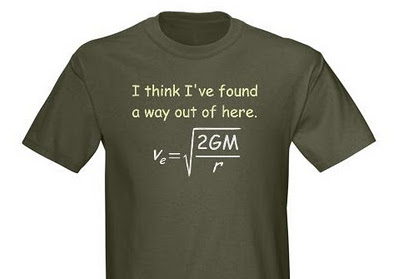
\includegraphics[scale=.4]{imagenes/velocidad_escape.jpg}
\end{center}

\end{frame}


\begin{frame}{Curvas de persecución}
 
\textbf{Problema} Supongamos que un conejo se mueve sobre una 
línea recta con rapidez uniforme $a$ y de un punto por fuera de la recta parte un perro que lo 
persigue con rapidez uniforme $b$. Encontrar la trayectoria del perrro
 
\begin{center}
\animategraphics[controls, scale=.4]{15}{pursuit/pursuit-}{0}{40}
\end{center}

 
 
 
\end{frame}

\begin{frame}{Curvas de persecución}
 \begin{tabular}{m{4.5cm} m{5cm}}
Supongamos que el perro parte del punto $(c,0)$, el conejo de $(0,0 )$ y la recta sobre la cual se mueve el conejo en dirección positiva  es el eje $y$. 
Vamos a suponer que la trayectoria del perro sigue la trayectoria tal que 
la tangente a su movimiento en un momento dado intersecta a la posición del conejo correspondiente a ese momento.
& 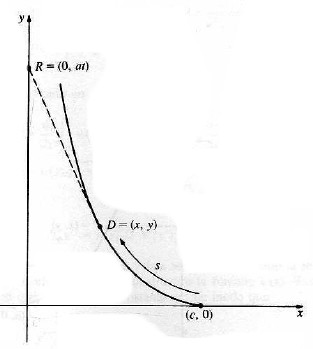
\includegraphics[scale=.4]{imagenes/persecucion.jpg}
\end{tabular}
\end{frame}


\begin{frame}{Curvas de persecución}
Pasado un tiempo $t$, el conejo estará en el punto $(0,at)$ y el perro en un punto de su trayectoria que forma un arco de
 longitud $s=bt$ hasta el $(c,0)$. Ese punto, donde está el perro, lo denotaremos $(x,y)$. Como hemos supuesto que la tangente a la trayectoria del perro en $(x,y)$ pasa 
 por la posición del conejo $(0,at)$ se debe cumplir que
 \begin{equation}\label{eq:persec}\frac{dy}{dx}=\frac{y-at}{x}\Longrightarrow xy'-y=-at.\end{equation}
 En esta ecuación hay tres variables, $t$ , $x$ e $y$. No es muy claro cuales estamos usando como independiente y cuales depenientes. 
 Generalmente el tiempo $t$ es una variable  indepeniente, pero en la expresión de arriba aparece la derivada de $y$ respecto a $x$. 
\end{frame}

\begin{frame}{Curvas de persecución}
  Pareciese como 
 que estamos considerando   $y$ tanto función de $t$ como de $x$. La intuición nos dice que $y$ la puedo pensar tanto como función de una u otra.
 
 Tratemos de elinar $t$ de esa ecuación, de modo de tener una ecuación, una variable dependiente y una independiente, como el Dios de la matemática manda.
 
  No es razonable pensar que lograremos tener menos variables sin pagar algún precio, pues, como dice el dicho, 
 \href{http://es.answers.yahoo.com/question/index?qid=20081023132736AABMX0}{``Cuando la limosna es grande hasta el santo desconfía'' }. 
\end{frame}

\begin{frame}{Curvas de persecución}
 En este caso, el costo que pagaremos 
 es incrementar el orden de la ecuación. 
 Como hemos dado algunas técnicas de  resolver ecuaciones de orden dos quizás estemos en condiciones de pagar este precio.
 
Para eliminar $t$ de la ecuación derivamos $\eqref{eq:persec}$ respecto a $x$. Queda
\[xy''=-a\frac{dt}{dx}.\]
Como $ds/dt=b$ 
\[\frac{dt}{dx}=\frac{dt}{ds}\frac{ds}{dx}=-\frac{\sqrt{1+y'(x)^2}}{b}.\]
El signo menos aparece porque $s$ es decreciente con $x$ pues $s=\int_x^c\sqrt{1+y'^2}dx$.
 
\end{frame}

\begin{frame}{Curvas de persecución}
 Entonces 
 \boxedeq{xy''=\frac{a\sqrt{1+y'(x)^2}}{b}.}
 
Que es una ecuación que no contiene $y$. De modo que usando $p=y'$ como variable dependiente reducimos el orden de la ecuación. Nos queda
\[\frac{dp}{\sqrt{1+p^2}}=\frac{a}{b}\frac{dx}{x}.\]
Que es una ecuación en variable separables. Tomando la integral definida entre $c$ y $x$, y considerando que si $x=c$ entonces $p=0$, tenemos
\[\ln\left(p+\sqrt{1+p^2}\right)=\ln\left( \frac{x}{c}\right)^{\tfrac{a}{b}}.\]
 
 
\end{frame}

\begin{frame}{Curvas de persecución}

Si despejamos $p$ queda

\boxedeq{p=\frac{dy}{dx}=\frac{1}{2}\left[\left(\frac{x}{c}\right)^{a/b}-\left(\frac{c}{x}\right)^{a/b}\right].}

Vamos a dejar que la continuidad del análisis como ejercicio.
 
 
\end{frame}

\begin{frame}{Oscilador armónico}\label{resortito}

\begin{tabular}{m{6cm} m{2cm}}
 Un \href{http://es.wikipedia.org/wiki/Oscilador_armónico}{oscilador armónico} es el más simple de los sistemas físicos vibratorios. Podemos definirlo como un sistema
elástico que obedece a la \href{http://es.wikipedia.org/wiki/Ley_de_Hooke}{Ley de elasticidad de Hooke}, en honor a su descubridor 
\href{http://es.wikipedia.org/wiki/Robert_Hooke}{Robert Hooke} & 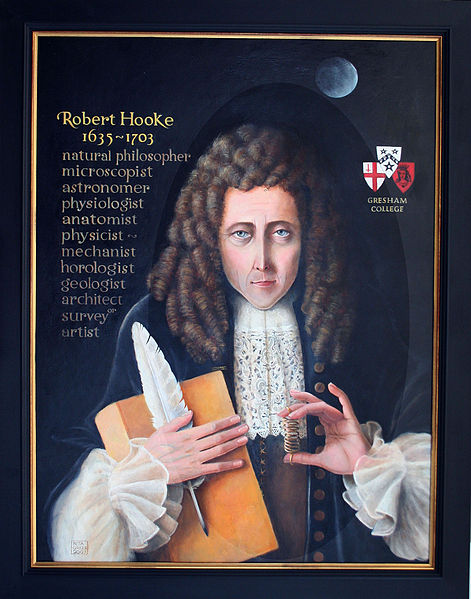
\includegraphics[scale=.15]{imagenes/Hooke.JPG}\\
\end{tabular}

 
\end{frame}

\begin{frame}{Oscilador armónico}\label{resortito}

\begin{center}
\animategraphics[controls, scale=.4]{15}{resorte/resorte-}{0}{47}
\end{center}
 
\end{frame}

\begin{frame}{Oscilador armónico}
Suele citarse al \href{http://es.wikipedia.org/wiki/Resorte}{resorte} como un ejemplo familiar de oscilador armónico.

Esto debido a que, cuando las oscilaciones de un resorte son
pequeñas,  se satisface aproximadamente la Ley de elasticidad de  Hooke.

Esta ley  afirma que la fuerza que ejerce un resorte sobre una masa $m$ conectada a él por uno 
de sus extremos es proporcional en magnitud al desplazamiento
del resorte desde la posición de equilibrio.

Además la fuerza de elasticidad actúa en sentido opuesto al desplazamiento
 
\end{frame}


\begin{frame}{Oscilador armónico}
 Supongamos que tenemos un resorte, en unos de sus extremos fijado en una pared y unido a una masa $m$ por el otro extremo. Supongamos que no actúa otra fuerza 
 sobre la masa. Ver la animación de pag. \ref{resortito}.  Pongamos un eje de coordenadas en la dirección del movimiento, con origen en la posición de equilibrio 
 del resorte. Esta posición es el punto donde el resorte no ejerce fuerza. Supongamos que la dirección positiva es la dirección donde el resorte se expande. Denotemos 
 por $x(t)$ la posición de la masa en el momento $t$.  

\end{frame}
\begin{frame}{Oscilador armónico}
  Entonces según la Segunda Ley de Newton y la Ley de Elasticidad de Hooke, tenemos que
 
 \boxedeq{mx''(t)=-kx(t).}{eq:resorte}
 
La constante de proporcionalidad $k$ se llama \href{http://es.wikipedia.org/wiki/Rigidez}{constante elástica}. La ecuación \eqref{eq:resorte} se denomina la
ecuación del oscilador armónico o ecuación del resorte.

\end{frame}

\begin{frame}{Oscilador armónico}

La ecuación del oscilador armónico se escribe $0=f(t,x,x',x'')$, donde en $f(t,x,y,z)=kx+mz$ es independiente de $t$. Podemos intentar usar $x$ como variable 
independiente y $z=x'$ como dependiente. Como vimos en la página \ref{reduc_orden} $x''(t)=dz/dt=dz/dx z$. Así la ecuación queda
\[\begin{split}
   m\frac{dz}{dx}z=-kx &\Longrightarrow mzdz=-kxdx\Longrightarrow m\frac{z^2}{2}=-k\frac{x^2}{2}+C_1\\
   &\Longrightarrow z=\pm\sqrt{-\frac{k}{m}x^2+C_1}\\
   &\Longrightarrow x'(t)=\pm\sqrt{-\frac{k}{m}x^2+C_1}.\\
  \end{split}
\]


\end{frame}


\begin{frame}{Oscilador armónico}
Debe ser $C_1\geq 0$ de lo contrario el dominio de la función sería vacío. Nos queda una nueva ecuación para $x'$.
Esta ecuación es en variables separables
\[ \frac{dx}{\sqrt{-\frac{k}{m}x^2+C_1}}=dt.   
\]

\end{frame}

\begin{frame}{Oscilador armónico}
 Integrando
\[\begin{split}
   t+C_2 
   &=\int \frac{dx}{\sqrt{-\frac{k}{m}x^2+C_1}}\\
   &= \sqrt{\frac{1}{C_1}} \int \frac{dx}{\sqrt{-\frac{k}{C_1m}x^2+1}} \\  
   &= \sqrt{\frac{m}{k}} \int \frac{du}{\sqrt{1-u^2}}\quad \left(\text{haciendo } u=\sqrt{\frac{k}{C_1m}}x\right)\\ 
   &=\sqrt{\frac{m}{k}}\arcsen u.
  \end{split}
\]
\end{frame}

\begin{frame}{Oscilador armónico}
Entonces
\[\begin{split}
    x=\frac{C_1m}{k}u &=\frac{C_1m}{k}\sen \left(\sqrt{\frac{k}{m}}(t+C_2)\right)\\
    &=\boxed{C_3\sen \sqrt{\frac{k}{m}}t+C_4\cos \sqrt{\frac{k}{m}}t}.
  \end{split}
 \]

Que es la solución general de la ecuación del oscilador armónico. Como vemos el movimiento es oscilatorio con frecuencia
\[\boxed{f=\sqrt{\frac{k}{m}} }.\]
En particular, no importan las condiciones iniciales, la frecuencia es siempre la misma. 

 
 

\end{frame}

\begin{frame}{EDP, método características}

\onslide<+->Saber resolver ecuaciones ordinarias de primer orden nos permite resolver algunas ecuaciones en derivadas parciales de primer orden. 

\onslide<+->Para tener un problema bien planteado con una ecuación en derivadas parciales no es suficiente conocer el valor de la función en un punto (como en una EDO de primer orden). En cambio una condición típica es dar el valor de la función a lo largo de una recta. 

\onslide<+-> Por ejemplo

\begin{equation}\label{eq:EDP_gral_1orden}
  \left.\begin{array}{l}
  a(x,y)u_x+b(x,y)u_y=c(x,y,u)\\
  u(x,0)=f(x)\\
\end{array}\right\}
\end{equation}
Aquí $x,y$ son variables independientes y $u$ dependiente.


 

\end{frame}

\begin{frame}{EDP, método características}

\onslide<+-> El método de características consiste en encotrar $u$ a lo largo de las soluciones de la ecuación

\boxedeq{\frac{dy}{dx}=\frac{b(x,y)}{a(x,y)}}{eq:ecua_caract}

\onslide<+-> Una solución de esta ecuación es normalmente una curva en el plano  $x,y$. La idea es que las soluciones de \eqref{eq:ecua_caract} forman un flia uniparamétrica
 de curvas que llena una gran parte $\Omega$ del plano $x,y$.  Así terminamos conociendo el valor de $u$ sobre este conjunto $\Omega$ 

\onslide<+-> Para que \eqref{eq:ecua_caract} tenga sentido debemos tener $a\neq 0$. De todas formas si $a=0$ podemos invertir los papales de $x$ e $y$.
\end{frame}

\begin{frame}{EDP, método características}


\onslide<+-> Supongamos $y(x)$ solución de \eqref{eq:ecua_caract}, entonces pongamos por abuso de notación $u(x)=u(x,y(x))$. Se tiene que

\boxedeq{\frac{du}{dx}=u_x+u_yy'=u_x+u_y\frac{b}{a}=\frac{c(x,y(x),u(x))}{a(x,y)}}{eq:ecua_caract2}
Que es otra ecuación ordinaria. Podemos escribir  \eqref{eq:ecua_caract} y \eqref{eq:ecua_caract2} en una ecuación más simétrica
\boxedeq{\frac{du}{c}=\frac{dx}{a}=\frac{dy}{b}}{eq:caract}


 
 \end{frame}

\begin{frame}{EDP, método características}


Estas ecuaciones se llaman \emph{ecuaciones características}. Las soluciones de estas ecuaciones son un familia de curvas que suele llenar un conjunto abierto de  $\mathbb{R}^3$. 

 La gráfica de la solución se obtine eligiendo de estas curvas las que pasan por $(x,0,f(x))$. Esto, en los casos favorables, forma una superficie que es la gráfica de la solución. La proyección de estas curvas en el plano $x,y$ se denominan \emph{caracterísitcas}. Son la familia de soluciones de $y'=b/a$.

\end{frame}

\begin{frame}{EDP, método características}

\textbf{Ejemplo:} Resolver
\begin{equation}\label{eq:EDP_gral_1orden}
  \left.\begin{array}{l}
  u_x+u_y=yu\\
  u(x,0)=f(x)\\
\end{array}\right\}
\end{equation}
En este caso
\[\frac{dy}{dx}=\frac{b}{a}\Rightarrow y'=1\Rightarrow y(x)=x+\mu,\quad\mu=\hbox{cte}.\]
Entonces
\[\frac{du}{dx}=\frac{c}{a}\Rightarrow u'=yu=(x+\mu)u\Rightarrow \ln|u|=\frac{x^2}{2}+\mu x+C(\mu).\]
Notar que la nueva constante de integración $C(\mu)$ debe depender de la primera $\mu$. Entonces
\[u=\pm e^{\frac{x^2}{2}}e^{(y-x)x}e^{C(y-x)}.\]

\end{frame}

\begin{frame}{EDP, método características}

Ahora
\[u(x,0)=f(x)\Rightarrow f(x)=\pm e^{\frac{x^2}{2}}e^{(-x^2}e^{C(-x)}\Rightarrow C(\mu)=\frac{\mu^2}{2}+\ln|f(-\mu)|.\]

Entonces

\[u(x,y)=\pm e^{\frac{x^2}{2}}e^{(y-x)x}e^{\frac{(y-x)^2}{2}+\ln|f(x-y)|        }
=e^{\frac{y^2}{2}}f(x-y).\]



\end{frame}

\end{document}
